% Chapter 1

\chapter{Attività di Stage} % Main chapter title

\label{Chapter3} % For referencing the chapter elsewhere, use \ref{Chapter1} 

\lhead{Capitolo 3. \emph{Attività di stage}} % This is for the header on each page - perhaps a shortened title

%----------------------------------------------------------------------------------------

\section{Pianificazione}

Viene di seguito riportato un diagramma di Gantt riassuntivo della pianificazione
del lavoro nel periodo di stage. Come si può vedere le ore sono state suddivise secondo
2 obiettivi, che rappresentano parti di sistema indipendenti che verranno sviluppate
in maniera autonoma.

GRAFICO

Il modello di ciclo di vita prescelto può essere paragonabile allo scrum: viene infatti preferito rispetto alla rigidità dei modelli più classici, in
quanto permetteva lo sviluppo continuo dei vari incrementi e la possibilità di mostrare
passo per passo i risultati ottenuti. Per chiarezza si riporta una breve descrizione degli
obiettivi presenti nel piano di lavoro che verranno maggiormente approfonditi nelle
sezioni successive:

\textbf{Obiettivo 1}: Creazione di una libreria che permetta il riconoscimento facciale\\
\textbf{Obiettivo 2}: Creazione di una libreria che permetta una facile condivisione dei contenuti multimediali eventualmente creati verso i social network


%----------------------------------------------------------------------------------------

\section{Analisi}

In seguito allo studio del dominio applicativo effettuato durante le prime ? settimane di stage e alle spiegazioni del tutor aziendale sono stati individuati i requisiti del prototipo richiesto.
Dal momento che si tratta di un prototipo che dovrà essere alla base di una famiglia di prodotti, esso non sarà indipendente dall input umano ma dovrà garantire la flessibilità ed espandibilità necessaria.

Di seguito vengono riportati i casi d'uso principali individuati.

\subsection{Casi d'uso}

Il caso d'uso è un tecnica usata nei processi di ingegneria del software per effettuare in maniera esaustiva e non ambigua, la raccolta dei requisiti funzionali al fine di produrre software di qualità.
Essa consiste nel valutare ogni requisito focalizzandosi sugli attori che interagiscono col sistema, valutandone le varie interazioni. Nel caso specifico, l'attore
principale è uno solo, ossia l'utente che utilizza il dispositivo mobile.

\textbf{UC1 Caso d'uso generale}
\\
\textbf{Precondizione:}
\\
\textbf{Postcondizione:}
\\
\textbf{Scenario principale:}
\\
GRAFICO UML
\\


\textbf{UC2 Caso d'uso generale}
\\
\textbf{Precondizione:}
\\
\textbf{Postcondizione:}
\\
\textbf{Scenario principale:}
\\
GRAFICO UML
\\


\textbf{UCx Caso d'uso generale}
\\
\textbf{Precondizione:}
\\
\textbf{Postcondizione:}
\\
\textbf{Scenario principale:}
\\
GRAFICO UML
\\

\subsection{Requisiti}



La classificazione dei requisiti sarà seguirà il formalismo:
\begin{center}
	\textbf{R\{TIPO\}\{RICHIESTA\}\{GERARCHIA\}}
\end{center}

Nello specifico:
\begin{itemize}
\item TIPO può essere:
	\begin{itemize}
		\item F, indica un requisito funzionale
		\item Q, indica un requisito di qualità
		\item V, indica un requisito di vincolo
	\end{itemize} 
\item IMPEGNO può essere:
	\begin{itemize}
		\item O, indica un requisito obbligatorio
		\item D, indica un requisito desiderabile
	\end{itemize} 
\item GERARCHIA: i requisiti sono organizzati gerarchicamente secondo una struttura ad albero. Se la complessità di un requisito viene ritenuta elevata, questo può essere diviso in sotto-requisiti.
\end{itemize}

A seguire i requisiti individuati:

\begin{center}
    \begin{tabular}{ | p{3cm} | l | p{3cm} |}
    \hline
    Requisiti & Descrizione & Caso d'uso \\ \hline
    test & test & test  \\ \hline 
    test & test & test \\ \hline
    test & test & test  \\ \hline 
    test & test & test \\ \hline
    test & test & test  \\ \hline 
    test & test & test \\ \hline
    test & test & test  \\ \hline 
    test & test & test \\ \hline
    \end{tabular}
\end{center}

\subsubsection{Modello di ciclo di vita}
%----------------------------------------------------------------------------------------

\section{Progettazione}

\subsection{Architettura}
\subsection{Tecnologie utilizzate}

\subsubsection{Java}

Il linguaggio per applicazioni Android è in realtà un "dialetto" del linguaggio Java così come è diversa anche la virtual machine di runtime (Dalvik virtual machine anziché JVM).
In una normale applicazione Android non c'è un entry point (il classico metodo "main") da dove normalmente un programma comincia a caricare le sue parti software e avviarsi: tutto è pensato per essere un "componente" pilotato dagli eventi ("Event Driven") dell'hardware o di altri componenti. Questo paradigma fa sì che il programmatore sviluppi per ogni hardware delle routine il più possibile indipendenti. Un vantaggio è che il sistema operativo potrà ottimizzare le risorse, ad esempio rinunciando a caricare componenti (e hardware) non supportati o non prioritari perché inutilizzati.


\subsubsection{Android NDK}

L NDK (Native Development Kit) è uno strumento che permette di implementare parte dell'applicazione usando codice scritto in linguaggio nativo come il C ed il C++. Per alcune applicazioni può essere utile in quanto si può riutilizzare le librerie scritte in tali linguaggi. L'uso di tale strumento non da però beneficio per la maggior parte delle applicazioni ed è da usare quindi con parsimonia (spesso l'aumento delle performance dovuto all'utilizzo di codice nativo non giustifica l'aumento di complessità). Tipicamente buoni candidati sono programmi che sono CPU-intensive che non allocano molta memoria come simulazioni fisiche ed analisi dei segnali. Nel caso specifico sono stati effettuati dei test per verificare se la quantità di chiamate verso la libreria C/C++ OpenCV giustifica tale strumento. 

\subsubsection{Android SDK}

Le applicazioni di Android sono sviluppate all'interno di un framework, ossia di una struttura dati specifica. La struttura del framework è molto chiara se si utilizza l'ambiente di sviluppo (Android SDK) con Eclipse; il mancato utilizzo di Eclipse, tuttavia, non impedisce di scrivere applicazioni Android funzionanti.
Le applicazioni Android sono caratterizzate da una certa dualità: parti dinamiche scritte in Java e parti statiche scritte in XML. Tipico delle parti statiche possono essere quelle caratteristiche che non cambiano durante l'esecuzione dell'applicazione, come per esempio il colore dello sfondo. Tipico delle parti dinamiche sono invece gli aspetti programmatici come per esempio la gestione degli eventi.
Questa dualità è però solo apparente. Durante l'esecuzione, infatti, l'ambiente di esecuzione o run-time noto come Dalvik virtual machine (DVM), che in tale ambito sostituisce la consueta Macchina virtuale Java (JVM), esegue sempre un programma. Per lo sviluppo delle applicazioni è disponibile una completa documentazione[98] la quale, anche graficamente, riprende la struttura tipica della documentazione Java[99] del sito Oracle.

Tramite l'SDK possiamo passare dalla descrizione della nostra applicazione alla sua effettiva esecuzione sia in emulazione, sia su un dispositivo concreto. Per descrivere l'applicazione al dispositivo prescelto si utilizza il file Manifest.xml. Possiamo quindi affermare che un'applicazione è descritta completamente da una tripletta:

\begin{itemize}
\item Codice Java
\item Risorse statiche xml
\item Manifest.xml
\end{itemize}

Il codice Java viene poi compilato insieme all'XML per generare un file con estensione .apk: esso contiene il bytecode per la cosiddetta Dalvik Virtual Machine (DVM). I passi successivi servono per installare il bytecode nel dispositivo (ed eseguirlo in emulazione).



\subsubsection{Android FD-Library}

All'interno delle SDK Android è presente una API per il riconoscimento facciale: Android.Media.FaceDetector. Questa classe permette, data un immagine, di trovare le eventuali facce presenti attraverso il semplice utilizzo del metodo findFaces(). Ogni istanza ritornata viene salvata in un array Faces[] e contiene:

\begin{itemize}
\item Valutazione se si tratta di un volto o meno 
\item Distanza tra gli occhi (numero di pixel)
\item Posizione (x,y) del punto medio situato tra i due occhi
\item Rotazioni di posa della faccia (x,y,z)
\end{itemize} 

A seguito di valutazioni e di un prototipo usa e getta si è però deciso di non utilizzare in quanto:

\begin{itemize}
\item Non ritorna il rettangolo che include con precisione la faccia

\item Non consente di utilizzare template a piacimento per la ricerca di feature specializzate (naso, occhi, orecchie, etc.)

\item Prestazioni discrete per una immagine unica, ma non adatta ad un applicazione real-time

\item Supporta solo bitmap in formato RGB\_565 

\item Sono stati rilevati comportamenti evidentemente diversi a seconda del dispositivo utilizzato, e la quantità di bug riportata dalla community Android è rilevante
\end{itemize}

\subsubsection{OpenCV}

OpenCV è una libreria creata da Intel a scopi di commerciali e di ricerca. E' una libreria open e gratuita, e pertanto il suo codice può essere utilizzato nella sua interezza o in parte. Al momento della stesura di questo documento la versione più recente disponibile è la v2.4.7 specifica per dispositivi Android. Tale versione fornisce un wrapper Java alle librerie OpenCV che fornisce quasi tutte le fonzionalità core. Al fine di garantire il funzionamento di applicativi basati su questa libreria è però necessario installare sul dispositivo un software chiamato OpenCV Manager, che permette all'applicazione ottimizzazioni in base all'hardware presente.

Vi sono due modi d'utilizzo di questa libreria:

\begin{itemize}
\item \textbf{Ad alto livello}:  utilizzo esclusivo delle Java API. Facilità di sviluppo, ma non permette l'accesso completo alle libreria. Prestazioni minori a causa al gran numero di chiamate JNI (Java Native Interface) verso la libreria

\item \textbf{A basso livello}:  utilizzo dell'interfaccia nativa di openCV. Android permette infatti di eseguire chiamate a funzioni native, ciò significa che è possibile utilizzare l'interfaccia C++ di OpenCV. 
\end{itemize}
%----------------------------------------------------------------------------------------





\subsection{Associazione classi-requisiti}


\section{Implementazione}



%----------------------------------------------------------------------------------------

\section{Verifica e validazione}

\subsection{Analisi Statica}
Al fine di portare avanti il processo di verifica con metodo è stato necessario renderlo
quantificabile. Perciò si sono definite delle metriche sul codice sorgente. Esse sono
di seguito definite e il loro significato viene descritto e spiegato. Per ogni metrica si
sono definiti un range di accettazione e un range ottimale.

\subsubsection{Complessità ciclomatica}

Tale metrica indica il numero di cammini linearmente indipendenti percorribili durante
l'esecuzione di un singolo metodo. Tale metrica è molto importante in quanto ha
implicazioni dirette sulle attività di testing: infatti essa rappresenta un upper bound
per il numero di routine di test necessarie per raggiungere un completo branch coverage.

\textbf{Range dichiarato:}
\begin{itemize}
\item Accettazione $\leq 15$
\item Ottimale $\leq 10$
\end{itemize}

\subsubsection{LOC}

Tale metrica (Lines of Code, linee di codice) indica il numero di linee di codice. Nel conteggio vengono escluse le righe contenenti dichiarazioni di namespaces, tipi, campi, metodi oltre che i metodi astratti e i tipi enumeration.
Solo il codice effettivamente eseguito è considerato nel conteggio delle righe.
La metrica LOC non è sempre legata alla produttività del programmatore, ma torna
utile sia nel calcolo della percentuale di statement coverage e nella valutazione del
software.
Essa è indice di manutenibilià (è più semplice manutenere metodi brevi) e quindi
qualità del codice.

\textbf{Range per metodo:}
\begin{itemize}
\item Accettazione $\leq 45$
\item Ottimale $\leq 15$
\end{itemize}

\subsubsection{Numero di campi utilizzati per classe}

Indica il numero di membri di classe (campi dati) di una particolare classe. E'
importante in quanto è indice delle responsabilità andate ad una classe, se viene
superato può indicare che la classe ne raggruppa troppe altre e andrebbe ulteriormente
separata in classi distinte.

\textbf{Range dichiarato:}
\begin{itemize}
\item Accettazione $\leq 16$
\item Ottimale $\leq 8$
\end{itemize}

\subsubsection{Numero di metodi utilizzati per classe}

Indica il numero di metodi di una particolare classe. Similmente al numero di campi
per classe è importante in quanto è indice delle responsabilità andate ad una classe, se
viene superato può indicare che la classe ha troppe funzionalità e andrebbe separata.

\textbf{Range dichiarato:}
\begin{itemize}
\item Accettazione $\leq 16$
\item Ottimale $\leq 8$
\end{itemize}

\subsubsection{LCOM e LCOM HS}

Si vuole definire una metrica a partire da questa definizione: se una classe ha una sola responsabilità si
dice che essa è coesa. In generale una classe risulterà coesa se i suoi metodi sono
strettamente legati fra loro. Quando metodi distinti non usano attributi o metodi
comuni significa che essi non condividono nulla e che quindi potrebbero venir separati.
La metrica di LCOM misura quindi quanto poco una classe è coesa. Alcune formule per il
calcolo di LCOM sono le seguenti:

\begin{center}
\textbf{LCOM} =  $1-(\sum(MF)/M \ast F) $  \\
\textbf{LCOM HS} = $(M-(\sum(MF)/F))\ast(M-1)$
\end{center}

Dove:
\begin{itemize}
\item M è il numero di metodi nella classe. Si considerano sia i metodi statici sia quelli di istanza, ed include inoltre i costruttori,getters e setters ed eventuali metodi del tipo add/remove
\item F è il numero di campi dati d'istanza all'interno della classe 
\item MF è il numero di metodi della classe che accedono un particolare campo dati di tipo classe
\item $\sum(MF)$ è la somma degli MF tra tutti i campi d'istanza della classe
\end{itemize}

L'idea alla base di tali formule è che una classe perfettamente coesa utilizza tutti i
suoi campi dati di tipo classe all'interno di ogni suo metodo il che comporta :

\begin{center}
 $(\sum(MF) = M \ast F) \Leftrightarrow LCOM = 0 $
\end{center}



La differenza tra LCOM e la sua versione HS (Hendersons-Sellers) è che la prima
ritorna dei valori nel range [0-1] mentre la seconda nel range [1-2]. La versione HS è
considerata più efficace per la rilevazione dei tipi scarsamente coesi.
Tale metrica è interessante, ma va trattata con cautela (basti pensare una classe
che ha n campi dati, n getters e n setters, essa risulterà scarsamente coesa, il che
non rispecchia la realtà). Infatti essa non va valutata singolarmente, ma deve essere
inserita in un contesto di valutazione che comprende altre variabili, soprattutto il
numero di campi e il numero di metodi. 

\textbf{Range dichiarato:}
\begin{itemize}
\item Accettazione $\leq 0.8$
\item Ottimale = 0
\end{itemize}


\subsection{Analisi Dinamica}
\subsection{Test di Validazione}

\section{Esiti attività}

\section{Valutazione prestazioni}

Al fine di verificare le prestazioni ottenute in media dall'applicativo, l'azienda ha fornito 4 dispositivi che rappresentano all'anno della stesura di questo documento (2014) le possibili fasce di mercato.

I dispositivi forniti sono:

\begin{itemize}
\item \textbf{Fascia Alta - \textit{Galaxy S4}} 
	\begin{itemize}
		\item CPU quad core 1.6GHz Cortex A15 
		\item RAM 2 GB 
		\item Fotocamera : posteriore: 13 MP , anteriore 2.1 MP
		\item Android 4.2.2 Jelly Bean 
	\end{itemize}
\item \textbf{Fascia Media - \textit{Galaxy S3 Mini}}
	\begin{itemize}
		\item CPU 1 GHz dual core ARM Cortex A9
		\item RAM 1 GB 
		\item Fotocamera : posteriore: 5 MP , anteriore 1 MP
		\item Android 4.1.1 Jelly Bean 
	\end{itemize}
\item \textbf{Fascia Bassa - \textit{Galaxy S}}
	\begin{itemize}
		\item CPU 0.8 GHz single core ARM Cortex A9
		\item RAM 1 GB 
		\item Fotocamera : anteriore 0.8 MP
		\item Android 2.3.0 Gingerbread
	\end{itemize}
\end{itemize}

Dal momento che le prestazioni possono dipendere dalla qualità della luce e dalla distanza dell utente dal dispositivo, si è preferito testare l'applicazione utilizzando video come input. Le variabili da tenere in considerazione sono risoluzione, numero di volti , numero di falsi positivi, numero di fotogrammi medi per secondo al termine di ogni video. I video sono sono volutamente caratterizzati da camere mobili, e da scene in cui non sono presenti persone al fine di verifica la presenza di falsi positivi.

I video utilizzati sono reperibili direttamente dal web ai link:

\begin{itemize}
\item[•] \href{http://www.youtube.com/watch?v=IIdGxR-aU6o}{Video 1}
\item[•] \href{http://www.youtube.com/watch?v=yWPyRSURYFQ}{Video 2}
\item[•] \href{http://www.youtube.com/watch?v=sL7cqpIvvRk}{Video 3}
\end{itemize}

Risoluzioni utilizzate:

\begin{itemize}
\item[•] $1280\ast960$ 
\item[•] $640\ast480$ 
\item[•] $320\ast240$ 
\end{itemize}

I seguenti test sono stati effettuati con parametri i seguenti parametri:
\begin{itemize}
\item \textit{FdActivity::mMinNeighbors} = 3 (sono necessari almeno 3 hit per frame per confermare positivamente il volto)
\item \textit{FdActivity::mMinSize} = -1  
\item \textit{FdActivity::mMaxSize} = -1
\item \textit{FdActivity::mScaleFactor} = 1.0 
\end{itemize}

In questo modo ci si assicura che il costo computazionale per ogni frame sia massimo (il metodo di riconoscimento facciale terminerà solo dopo aver valutato l'immagine nella sua interezza). 
Dato che per ogni singolo frame vi possono essere più hits corrispondenti allo stesso volto, è stata creata una semplice funzione ad hoc che permetta di contare un solo volto per set coincidenti di hits. 

\begin{figure}[h]\centering  
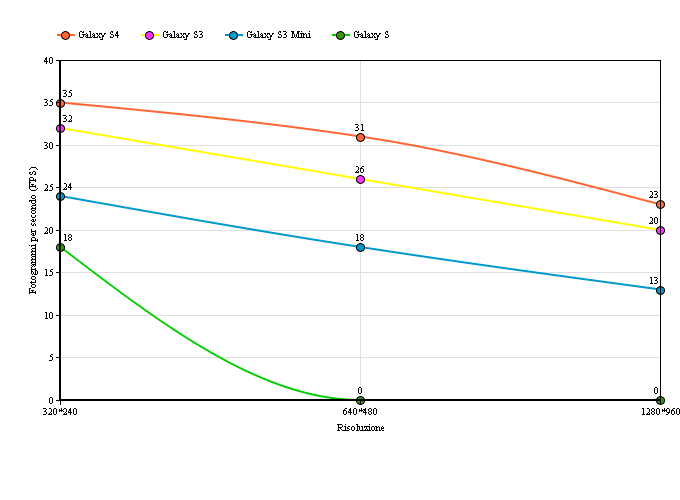
\includegraphics[scale=0.6]{../Figures/graph_1.png}
\caption[Long caption]{Caption}
\label{pic-a}
\end{figure}

Al variare dei dispositivi non vi è alcuna differenza nei risultati (quantità di volti rilevati + $\varepsilon$(falsi positivi rilevati)) se non al variare del parametro \textit{FdActivity::mMinNeighbors}. Infatti,prendendo come risoluzione di riferimento $640 \ast 480$, sono stati ottenuti i seguenti risultati
\\
GRAFICO A RES FISSA CON NUM FALSI POSITIVI E NEGATIVI AL VARIARE DELLA RETENTION 
\\
I risultati sono però stati totalmente differenti nell'utilizzo reale utilizzando la fotocamera posteriore come input dei frame al posto dei video (che garantivano un framerate costante di 24 fotogrammi per secondo). 
\\
GRAFICO LUMINOSITA NORMALE

GRAFICO LUMINOSITA BASSA
\\
Infine si può notare come vi siano grosse discrepanze di prestazioni al variare della fotocamera d'input (Anteriore o Posteriore). Questo è dovuto al fatto che generalmente la fotocamera posteriore è di qualità maggiore (sensore di dimensioni maggiori, diaframma più aperto ed ISO che può raggiungere valori più elevati)
\\
GRAFICO FRONTALE VS POSTERIORE

\subsection{Considerazioni}

A seguito dei test effettuati l'idea è che i dispositivi correntemente presenti sul mercato abbiamo una potenza computazionale più che sufficiente per eseguire tali task con prestazioni discrete e garantiscano un'esperienza d'utilizzo adeguata. Il maggior problema riscontrato è sicuramente la qualità della fotocamera che può condizionare drasticamente le performance se posta in condizione d'utilizzo non ottimale. Il software preinstallato sullo smartphone infatti, in condizioni di bassa luminosità, tende ad alzare il valore ISO (sensibilità del sensore) ed ad utilizzare un diaframma il più aperto possibile. La necessità di miniaturizzare l'hardware fotografico ha però come conseguenza quella di non poter avere sensori e lenti di dimensioni adeguate. Questo si traduce in bassa qualità, e pertanto per ogni singolo frame di un video sarà necessario un tempo di esposizione molto elevato. Lo stream di fotogrammi risulterà quindi caratterizzato da un framerate molto basso, mettendo il processore in attesa attiva del fotogramma da processare. 


%----------------------------------------------------------------------------------------

